%2multibyte Version: 5.50.0.2953 CodePage: 1252

\documentclass[bigger,handout]{beamer}
%%%%%%%%%%%%%%%%%%%%%%%%%%%%%%%%%%%%%%%%%%%%%%%%%%%%%%%%%%%%%%%%%%%%%%%%%%%%%%%%%%%%%%%%%%%%%%%%%%%%%%%%%%%%%%%%%%%%%%%%%%%%%%%%%%%%%%%%%%%%%%%%%%%%%%%%%%%%%%%%%%%%%%%%%%%%%%%%%%%%%%%%%%%%%%%%%%%%%%%%%%%%%%%%%%%%%%%%%%%%%%%%%%%%%%%%%%%%%%%%%%%%%%%%%%%%
\usepackage{amssymb}
\usepackage{amsfonts}
\usepackage{amsmath}
\usepackage{mathpazo}
\usepackage{hyperref}
\usepackage{multimedia}
\usepackage{pgfpages}
\usepackage{graphicx}

\setcounter{MaxMatrixCols}{10}
%TCIDATA{OutputFilter=LATEX.DLL}
%TCIDATA{Version=5.50.0.2953}
%TCIDATA{Codepage=1252}
%TCIDATA{<META NAME="SaveForMode" CONTENT="1">}
%TCIDATA{BibliographyScheme=Manual}
%TCIDATA{Created=Monday, October 27, 2008 15:56:24}
%TCIDATA{LastRevised=Monday, February 27, 2012 20:44:16}
%TCIDATA{<META NAME="GraphicsSave" CONTENT="32">}
%TCIDATA{<META NAME="DocumentShell" CONTENT="Other Documents\SW\Slides - Beamer">}
%TCIDATA{Language=American English}
%TCIDATA{CSTFile=beamer.cst}

\newenvironment{stepenumerate}{\begin{enumerate}[<+->]}{\end{enumerate}}
\newenvironment{stepitemize}{\begin{itemize}[<+->]}{\end{itemize} }
\newenvironment{stepenumeratewithalert}{\begin{enumerate}[<+-| alert@+>]}{\end{enumerate}}
\newenvironment{stepitemizewithalert}{\begin{itemize}[<+-| alert@+>]}{\end{itemize} }
\usetheme{Madrid}
\usecolortheme{beaver}
\input{tcilatex}
\setbeamertemplate{navigation symbols}{}
\begin{document}

\title[47-809: Perturbation]{Perturbation}
\subtitle{Judd Chapter 13}
\author[David Childers]{David Childers (thanks to Y. Kryukov, K. Judd, and U. Doraszelski)}
\institute[CMU]{CMU, Tepper School of Business}
\date[Apr.-19]{April 19, 2023}
\maketitle

 
 
\begin{frame}%
 
\QTR{frametitle}{Perturbation method}

\begin{itemize}
\item Some models in Macro only need policy function \newline
near the steady state

\item This suggests Taylor series expansion around the steady state

\item Relies on Implicit Function Theorem

\item Another derivation-intensive method (formerly)

\item Now, with automatic differentiation, extremely easy
\end{itemize}

 
 
\end{frame}%
 
 
 
\begin{frame}%
 
\QTR{frametitle}{Implicit Function Theorem}

\begin{stepitemize}
\item We have $H(x,y):\mathbb{R}^{d_{x}}\times \mathbb{R}^{d_{y}}\rightarrow \mathbb{%
R}^{n}$; derivatives $H_{x}$, $H_{y}$

\item We want $h(x):\mathbb{R}^{d_{x}}\rightarrow \mathbb{R}^{d_{y}}$, but we only
know that: 
\begin{equation*}
H(x,h(x))=0
\end{equation*}

\item This implies that $\frac{d }{d x}H(x,h(x))=0$:%
\begin{equation*}
H_{x}\left( x,h(x)\right) +H_{y}\left( x,h(x)\right) h_{x}(x)=0
\end{equation*}

\item Imagine we know $x_{0}$ and $y_{0}=h\left( x_{0}\right) $. Then:%
\begin{equation*}
h_{x}(x_{0})=-\left[ H_{y}\left( x_{0},y_{0}\right) \right] ^{-1}H_{x}\left(
x_{0},y_{0}\right)
\end{equation*}

\item Linear approximation:%
\begin{equation*}
h^{L}(x)=h\left( x_{0}\right) +h_{x}\left( x_{0}\right) \left( x-x_{0}\right)
\end{equation*}

\item Quality check: $E=H(x,h^{L}(x))$
\end{stepitemize}

 
 
\end{frame}%
 
 
 
\begin{frame}%
 
\QTR{frametitle}{Higher-order implicit function}

\begin{stepitemize}
\item $\frac{d ^{2}}{d xx}H(x,h(x))=0$:%
\begin{eqnarray*}
\tfrac{d }{d x}\left[ H_{x}\left( x,h(x)\right) +H_{y}\left(
x,h(x)\right) h_{x}(x)\right] &=&0 \\
H_{xx}[.,.]+2H_{xy}[.,h_{x}[.]]+H_{yy}[h_{x}[.],h_{x}[.]]+H_{y}[h_{xx}[.,.]] &=&0
\end{eqnarray*}%
Note that $H_{ab}$ is a 3-dimensional array ($n \times d_{a} \times d_{b}$ tensor)

\item Let $H_{...}^{0}=H_{...}\left( x_{0},y_{0}\right) $, $%
h_{...}^{0}=h_{...}\left( x_{0}\right) $

\item Solve for $h_{xx}$ (using $h_{x}$ known from first order): 
\begin{equation*}
h_{xx}^{0}[,]=-\left[ H_{y}^{0}\right] ^{-1}\left(
H_{xx}^{0}[.,.]+2H_{xy}^{0}[.,h_{x}^{0}[.]]+H_{yy}^{0}[h_{x}^{0}[.],h_{x}^{0}[.]]\right)
\end{equation*}

\item Solve by flattening tensor to vector and solving linear system, or by iterative methods

\item Quadratic approximation:%
\begin{equation*}
h^{Q}(x)=h^{0}+h_{x}^{0}\left( x-x_{0}\right) +\tfrac{1}{2}\left(
x-x_{0}\right) ^{\top }h_{xx}^{0}\left( x-x_{0}\right)
\end{equation*}
\end{stepitemize}

 
 
\end{frame}%
 
 
 
\begin{frame}%
 
\QTR{frametitle}{Perturbation strategy}

\begin{stepitemize}
\item Formulate the problem as an implicit function.

\item Pick $x^{0}$ to make $y^{0}=h\left( x^{0}\right) $ easy to compute

\begin{stepitemize}
\item Deterministic dynamic models: steady state

\item Dynamic stochastic model: steady state becomes\newline
stable/stationary distribution

\item Assume zero shocks $\Rightarrow $ deterministic problem;\newline
steady state will be close to stationary mode at low noise.
\end{stepitemize}

\item Construct approximation

\item Check solution over full range of values\bigskip

\item Taylor approximation is limited by radius of convergence -- distance
to nearest singular point (any derivative unbounded)

% \item Taylor approximations to objective and constraints are an inferior
% (and older) method.
\end{stepitemize}

 
 
\end{frame}%


\begin{frame}%
 
\QTR{frametitle}{Recursive Models}

\begin{itemize}
\item Dynamic models often expressed in recursive form
\item Especially models w/ dynamic optimization
\item Perturbation approach requires setting up as differentiable system of equations
\begin{itemize}
\item Use Euler method or FOC approach to describe conditions
\end{itemize}
\item Combine many equations
\begin{itemize}
\item Multiple agent decisions (firms, consumers, gov)
\item Equilibrium constraints: market clearing, dynamic budget
\item Exogenous dynamics of shocks, policies, etc
\end{itemize}



\end{itemize}
\end{frame}%

\begin{frame}%
 
\QTR{frametitle}{Recursive Models}

\begin{itemize}
\item Discrete time recursive representation
\begin{equation*}
E_x F(x,y,x^{\prime},y^{\prime})=0
\end{equation*}
\item $y$ are "jump" variables: determined endogenously by $x$
\item $x=(x_1,x_2)$ are "predetermined" variables
\item $x_2$ evolves exogenously via $x_2^{\prime}=h_2(x_2)+\sigma\epsilon^{\prime}$
\item $\epsilon$ is mean 0, (only) source of stochastic shocks
\item May need to add variables to get model to fit format
\item \emph{Recursive} equilibrium is functions $g(x),h(x)=(h_1(x),h_2(x_2))$ s.t. $\forall x$
\begin{equation*}
E_x F(x,g(x),h(x)+\sigma\epsilon^{\prime},g(h(x)+\sigma\epsilon^{\prime}))=0
\end{equation*}
\item Nested structure calls for modified approach
\end{itemize}

\end{frame}%

\begin{frame}%
 
\QTR{frametitle}{Perturbation for Recursive Models}

\begin{itemize}
\item Expand around \emph{nonstochastic} steady state
\item Set $\sigma=0$ and find $x^*,y^*$ s.t. $x_2^{*}=h_2(x_2^{*})$ and
\begin{equation*}
F(x^{*},y^{*},x^{*},y^{*})=0
\end{equation*}
\item Find by nonlinear equation solver
\item Want Taylor expansion of $h,g$ in $x$ $\&$ $\sigma$
\begin{equation*}
g(x,\sigma)=y^{*}+g_{x}(x-x^{*})+g_{\sigma}\sigma +\ldots
\end{equation*}
\begin{equation*}
h(x,\sigma)=x^{*}+h_{x}(x-x^{*})+h_{\sigma}\sigma +\ldots
\end{equation*}
\item Derivative wrt $x,\sigma$ at $x^{*},0$ must be 0: Apply chain rule
\begin{equation} \label{xderiv}
F_{x}+F_{y}g_{x}+F_{x^{\prime}}h_{x}+F_{y^{\prime}}g_{x}h_{x}=0
\end{equation}
\begin{equation} \label{sigderiv}
E_x[F_{y}g_{\sigma}+F_{x^{\prime}}(h_{\sigma}+\epsilon^{\prime})+F_{y^{\prime}}(g_{x}(h_{\sigma}+\epsilon^{\prime})+g_{\sigma})]=0
\end{equation}

\end{itemize}

\end{frame}%

\begin{frame}%
 
\QTR{frametitle}{Solving the system}

\begin{itemize}
\item By 0 mean, can show \ref{sigderiv} implies $h_\sigma,g_\sigma=0$
\item Rewrite \ref{xderiv} in matrix form $A=\left[F_{x}, F_{y}\right]$, $B=-\left[F_{x^{\prime}}, F_{y^{\prime}}\right]$
\begin{equation} \label{systemsolve}
A \begin{bmatrix} 
I \\ 
g_x
\end{bmatrix} 
= B 
  \begin{bmatrix} 
I \\ 
g_x
\end{bmatrix} 
  \begin{bmatrix}
  h_{x} & 0 \\
   0 &   h_{x}
  \end{bmatrix}
\end{equation}
\item Matrix equation has many solutions: need additional conditions
\item Usually, model is BVP: require transversality
\item Sufficient condition: $h^{n}(x_0)\to x^{*}$ return to steady state
\item In linear case, means $h_{x}^{n}(x-x^{*})\to 0$
\begin{itemize}
\item Holds if $\max\left|\text{eig} (h_x)\right|<1$
\end{itemize}
\item Together, these conditions select a solution

\end{itemize}

\end{frame}%

\begin{frame}%
 
\QTR{frametitle}{Matrix Decomposition}

\begin{itemize}
\item To impose stability, break system into stable and unstable parts
\begin{itemize}
\item Align coordinates along stable vs unstable manifold
\end{itemize}
\item For linear system $x^{\prime}=Mx$, use diagonalization: Jordan decomposition
\item $M=U^{-1}DU$, $D$ (block) diagonal, eigenvalues along diagonal 
\item $\tilde{x}=Ux$ split into $1-d$ linear maps: solve in closed form
\item If $A$ invertible, can apply to $A^{-1}B$ (Blanchard Kahn method)
\item In general, $A$ noninvertible $\&$ decomposition numerically ill-posed
\item Solve both by \emph{Generalized Schur} (QZ) Decomposition $\left(A,B\right)=\left(QSU,QTU\right)$
\item $Q$, $U$ Unitary  $S$, $T$ block upper triangular
\item $U$ unitary means $U^{*}=U^{-1}$, $UU^{*}=I$, $U^{*}U=I$


\end{itemize}

\end{frame}%

\begin{frame}
\QTR{frametitle}{Applying Matrix Decomposition}

\begin{itemize}
\item QZ allows decomposing into blocks
\begin{equation*}
\left(S,T\right)=\left(
  \begin{bmatrix}
  S_{11} & S_{12} \\
   0 & S_{22}
  \end{bmatrix}
  ,
    \begin{bmatrix}
  T_{11} & T_{12} \\
   0 & T_{22}
  \end{bmatrix}
  \right)
\end{equation*}
\item Ordered so that $\max\left|\text{eig} (S_{11}^{-1}T_{11})\right|<1$
\item Applying Generalized Schur to \ref{systemsolve}, obtain
\begin{equation*}
QSU \begin{bmatrix}
I \\
g_x
\end{bmatrix}
= QTU
  \begin{bmatrix}
I \\
g_x
\end{bmatrix}
  \begin{bmatrix}
  h_{x} & 0 \\
   0 &   h_{x}
  \end{bmatrix}
\end{equation*}
\item Can remove $Q$ from both sides and decompose $U$ conformably
\begin{equation*}
\begin{bmatrix}
  S_{11} & S_{12} \\
   0 & S_{22}
  \end{bmatrix}
  \begin{bmatrix}
  U_{11} & U_{12} \\
   U_{21} & U_{22}
  \end{bmatrix}
 \begin{bmatrix}
I \\
g_x
\end{bmatrix}
=
\end{equation*}
\begin{equation*}
    \begin{bmatrix}
  T_{11} & T_{12} \\
   0 & T_{22}
  \end{bmatrix}
  \begin{bmatrix}
  U_{11} & U_{12} \\
   U_{21} & U_{22}
  \end{bmatrix}
  \begin{bmatrix}
I \\
g_x
\end{bmatrix}
  \begin{bmatrix}
  h_{x} & 0 \\
   0 &   h_{x}
  \end{bmatrix}
\end{equation*}






\end{itemize}

\end{frame}%


\begin{frame}
\QTR{frametitle}{Solution by Matrix Decomposition}

\begin{itemize}
\item Simplify
\begin{equation*}
\begin{bmatrix}
  S_{11} & S_{12} \\
   0 & S_{22}
  \end{bmatrix}
  \begin{bmatrix}
  U_{11} + U_{12}g_x \\
   U_{21} + U_{22}g_x
  \end{bmatrix}
=
    \begin{bmatrix}
  T_{11} & T_{12} \\
   0 & T_{22}
  \end{bmatrix}
  \begin{bmatrix}
  (U_{11}+ U_{12}g_x)h_x \\
   (U_{21} + U_{22}g_x)h_x
  \end{bmatrix}
\end{equation*}
\item Jump variables move so that system always on stable manifold
\item This is ensured if $g_x=-U_{22}^{-1}U_{21}$
\item Then second line is 0, and first line implies
\begin{equation*}
h_x=(U_{11} - U_{12}U_{22}^{-1}U_{21})^{-1}S_{11}^{-1}T_{11}(U_{11} - U_{12}U_{22}^{-1}U_{21})
\end{equation*}
\item By construction, $h_x$ satisfies stability
\item To do this, need $U_{22}^{-1}$ to exist: Blanchard-Kahn conditions 
\begin{itemize}
\item Map from unstable manifold to jump variables
\item $\#$ of jump variables equals $\#$ of eigenvalues $\geq 1$
\item If too many large eigenvalues, no non-explosive solutions
\item If too few first order info can't pin down unique solution
\end{itemize}


\end{itemize}

\end{frame}%


\begin{frame}
\QTR{frametitle}{Properties of linearized solution}

\begin{itemize}

\item Using above solutions, have linear approx to dynamics
\item Can calculate impulse responses, simulate forward, or estimate
\item Linear model allows VAR (if all observed) or linear state space model (if not) representation of system
  \begin{itemize}
  \item Gaussian shocks: construct likelihood by Kalman filter
  \item Likelihood-based estimation orders of magnitude faster if linear
  \end{itemize}
\item Cost of matrix calculations is $O(n^3)$ in number $n$ of equations
\item Compare: nonlinear methods can scale exponentially in $n$
  \begin{itemize}
  \item Curse of dimensionality reduced since only ask for local info
  \end{itemize}
\item Derivatives can be automatic or symbolic, canned routines exist
  \begin{itemize}
  \item Dynare, Schmitt-Grohe-Uribe, DSGE.jl, Gensys, even Stata
  \end{itemize}

\end{itemize}

\end{frame}%


\begin{frame}
\QTR{frametitle}{Going to Higher Order}
\begin{itemize}
\item Can extend to second and higher order analogously to above
\begin{equation*}
h(x,\sigma)\approx h(x^{*},0)+h_{x}(x-x^{*})+h_{\sigma}\sigma+\frac{1}{2}h_{xx}\left[x-x^{*},x-x^{*}\right]
\end{equation*}
\begin{equation*}
+h_{x\sigma}\left[x-x^{*},\sigma\right]+\frac{1}{2}h_{\sigma\sigma}\sigma^2+\ldots
\end{equation*}
\item Order $(k)$ derivatives found by taking derivatives of $E[F(x,g(x,\sigma),h(x,\sigma)+\sigma\epsilon,g(h(x,\sigma)+\sigma\epsilon,\sigma)]=0$
\item Equations in second derivatives based on second derivatives of system, first derivatives calculated by 1st order method
\item Solve this system for second derivatives, then use these in system to find third, etc
\item $2^{nd}$ $\&$ higher order methods result in \emph{linear} matrix equations





\end{itemize}

\end{frame}%

\begin{frame}
\QTR{frametitle}{Higher order perturbation}

\begin{itemize}
\item Simple to solve and no additional existence/uniqueness issues
\item But sytem dimension $O(n^{(k)})$ grows exponentially in order
\begin{itemize}
\item Have to stop at small to moderate order
\end{itemize}
\item Each order increases set of moments of shock that matter
\begin{itemize}
\item Linear solution \emph{certainty equivalent}
\item $\to$ Same coefs as if no shock at all
\item Variance starts to affect mean at order 2, Skewness at 3, etc
\item Need even higher orders for effect of moment to vary with $x$
\end{itemize}
\item Higher order perturbation good compromise if system dimension moderate but nonlinearities/interactions matter
\item May be unwieldy for estimation or simulation
\begin{itemize}
\item Likelihood methods need particle filter: slow
\item Simulations may fail to be stationary when true solution is
\item May need to "prune" higher order terms for reasonable behavior

\end{itemize}
% \begin{itemize}
% \item Nonlinear state space models challenging to estimate by likelihood methods
% \item Need large number of nested integrals: particle filter
% \item Simulation methods easier, but: 
% \item Simulations from quadratic or higher order models badly behaved
% \item Need not be stationary, even if exact solution is
% \item May need to "prune" higher order terms for well-behaved simulations
% \end{itemize}

\end{itemize}


\end{frame}


\begin{frame}
\QTR{frametitle}{When is perturbation feasible?}

\begin{itemize}

\item Need to be able to write system so differentiable
\begin{itemize}
    \item Often just algebra: Take FOCs to get rid of max
    \item Can fail with non-smooth model 
    \item Kinks, discontinuities, discrete variables all cause issues
    \item "Mixed" procedures exist for some of these: not always reliable
\end{itemize}  
\item Need nonstochastic steady state to exist
\item Existence usually not an issue: \emph{uniqueness} is
\item None of above improved by higher order solutions



\end{itemize}

\end{frame}%


\begin{frame}
\QTR{frametitle}{What if steady state nonunique?}

\begin{itemize}
\item If multiple isolated solutions, can choose 1, but may not be stable
  \begin{itemize}
  \item Nonlinear solution may involve moving between
  \item Even if BK conditions hold, only correct if true shocks bounded, keep system near 1 point
  \end{itemize}
  
\item May have continuum of steady states
\begin{itemize}
    \item Some variables not determined with no shocks
    \item E.g.: portfolio choice nonunique if all assets have 0 risk
    \item Can apply modified approach: bifurcation methods
    \item Hack: add small penalty function which differentiates choices
    \item Picks out unique choice, but maybe not same as in full nonlinear model 
\end{itemize}    

\end{itemize}

\end{frame}%






\begin{frame}
\QTR{frametitle}{Perturbation Approach: Pros and Cons}

\begin{itemize}
\item Way faster than projection for moderate order Taylor expansion (say $\leq 5$)
\item Also way easier to code, nearly completely automated
\item Especially suitable for high-dimensional models
\begin{itemize}
\item Method of choice for large DSGE models with many variables
\item In low-moderate dimensions, projection feasible and may be more accurate 
\end{itemize}
\item Con: accuracy low far from steady state
\item Major con: if no steady state, or many, completely misrepresents dynamic properties
\item Works poorly for models with kinks, jumps, multimodality, discreteness, etc
\begin{itemize}
\item Zero lower bound, borrowing constraint, regime switches, etc
\end{itemize}
\item Even if you plan to use global method, often good idea to start local to find initial guesses


\end{itemize}

\end{frame}%

\begin{frame}
\frametitle{Example: Stochastic Growth Model}
\begin{itemize}
\item Perturbation example and software implementation in Dynare
\begin{itemize}
\item From Collard, Juillard, Villemot (2009)
\end{itemize}
\item Representative consumer chooses consumption and labor to optimize
\begin{equation*}
\underset{(c_t,h_t)_{t=0}^{\infty}}{\max}E_{t}\sum_{t=0}^{\infty}\beta^{t}\log(c_t)-\theta\frac{h_t^{1+\psi}}{1+\psi}
\end{equation*}
\begin{equation*}
\text{s.t. }k_{t+1}=\exp(b_t)(y_t-c_t)+(1-\delta)k_t
\end{equation*}
\begin{equation*}
y_{t}=\exp(a_t)k_{t}^{\alpha}h_{t}^{1-\alpha}
\end{equation*}
\item with exogeneous shocks
\begin{equation*}
\begin{bmatrix} a_t \\ b_t \end{bmatrix} = 
\begin{bmatrix} \rho & \tau \\ \tau & \rho \end{bmatrix} +
\begin{bmatrix} \epsilon_t \\ \nu_t \end{bmatrix}
\end{equation*}
\begin{equation*}
\text{Cov}\begin{bmatrix} \epsilon_t \\ \nu_t \end{bmatrix} =
\begin{bmatrix} \sigma_\epsilon & \phi\sigma_\epsilon\sigma_\nu \\ \phi\sigma_\epsilon\sigma_\nu & \sigma_\nu \end{bmatrix}
\end{equation*}

\end{itemize}
\end{frame}


\begin{frame}
\frametitle{Implementation Steps}
\begin{itemize}
\item To solve by perturbation
\begin{enumerate}
\item Represent in terms of recursive differentiable equations
\item Solve nonlinear system for nonstochastic steady state
\item Differentiate to get first derivatives
\item Apply matrix decomposition to get first order solution
\item (Optional) Differentiate again and solve linear system to get next higher order
\item Repeat previous step as many times as desired
\end{enumerate}
\item Software takes care of steps (2)-(6), (1) usually manual


\end{itemize}
\end{frame}

\begin{frame}
\frametitle{Stochastic Growth Model: Equations}
\begin{itemize}
\item Step (1) here means deriving Euler equation and FOC for $h_t$

\begin{align*}
c_t\theta h_{t}^{1+\psi}=(1-\alpha)y_t \\
\beta E_t\left[\left(\frac{\exp(b_t)c_t}{\exp(b_{t+1})c_{t+1}}\right)\left(\exp(b_{t+1}\alpha\frac{y_{t+1}}{k_{t+1}}+1+\delta)\right)\right]=1 \\
y_{t}=\exp(a_t)k_{t}^{\alpha}h_{t}^{1-\alpha} \\
k_{t+1}=\exp(b_t)(y_t-c_t)+(1-\delta)k_t \\
a_t = \rho a_{t-1} + \tau b_{t-1} +\epsilon_t \\
b_t = \tau a_{t-1} + \rho b_{t-1} +\nu_t
\end{align*}

\item Code \emph{example1.mod} in Dynare or \emph{RBCPerturbation.ipynb} in \emph{DifferentiableStateSpaceModels.jl}
\begin{itemize}
\item Declares variables, params, starting value for nonlinear solver
\item Model then written as above
\item Declare order and run to simulate, get IRFs and moments
\end{itemize}
\begin{itemize}
\item Many options available to solve, estimate, etc: see user guides
\end{itemize}


\end{itemize}
\end{frame}


\begin{frame}
\frametitle{Stochastic Growth Model: IRFs for second order solution: epsilon}
\scalebox{0.5}{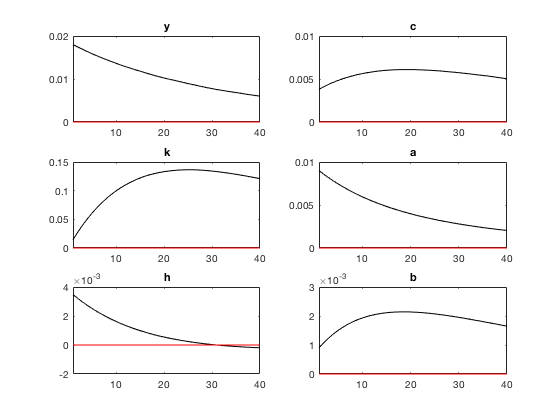
\includegraphics{order2shock_to_e.png}}

\end{frame}

\begin{frame}
\frametitle{Stochastic Growth Model: IRFs for second order solution: nu}
\scalebox{0.5}{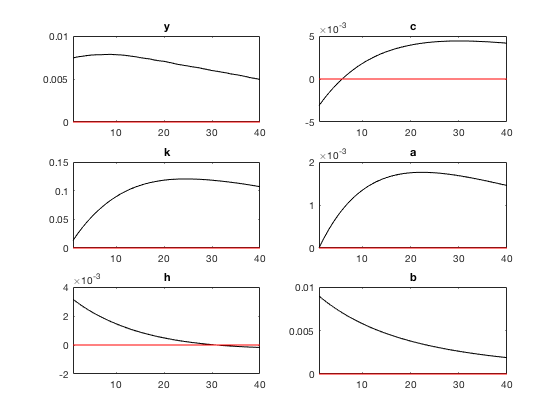
\includegraphics{order2shock_to_u.png}}

\end{frame}


\begin{frame}
\frametitle{Conclusions}
\begin{itemize}
\item Main advantage of perturbation is speed of coding
\item Well-maintained public libraries ensure speed, extensibility, follow-up analyses
\item Put together a model for your problem in a day or so
\begin{itemize}
\item Estimate it also in a weekend
\end{itemize}
\item Quickly iterate through models to check implications, compare against data, devise fixes and improvements
\item Goal of computation is to answer economic question
\begin{itemize}
\item Value comes from results, not methods
\item Use sophisticated methods when genuinely needed to produce answer
\end{itemize}


\end{itemize}

\end{frame}

\begin{frame}
\frametitle{References}

\begin{itemize}
\item Theory
\begin{itemize}
\item Judd Ch 13, Fer\'{a}ndez-Villaverde et al Handbook chapter
\end{itemize}
\item Software
\begin{itemize}
\item \href{https://www.dynare.org/}{Dynare}: extremely polished, full-featured. C++, optional Matlab, Julia interfaces 
\item \href{https://github.com/HighDimensionalEconLab/DifferentiableStateSpaceModels.jl}{DifferentiableStateSpaceModels.jl}: Adds autodiff features
\item Variants: Sims \href{http://sims.princeton.edu/yftp/gensys/}{gensys}, Uhlig Toolkit, \href{https://www1.columbia.edu/~ss3501/}{Schmitt-Grohe-Uribe}, \href{https://frbny-dsge.github.io/DSGE.jl/}{DSGE.jl}, etc
\end{itemize}
\item{Extensions}
\begin{itemize}
\item Continuous time: Sims (2002) "Solving linear rational expectations models"
\item Piecewise linear: Occbin (in Dynare)
\item $\infty$-dimensions: next class
\end{itemize}


\end{itemize}

\end{frame}



% \begin{frame}%
%  
% \QTR{frametitle}{Example: optimal growth (cont. time)}
% 
% \begin{stepitemize}
% \item Bellman equation:%
% \begin{equation}
% \rho V(k)=\max_{c}u\left( c\right) +V^{\prime }(k)\left[ f(k)-c\right]
% \label{eq_Bell}
% \end{equation}
% 
% \item Solution $C(k)$ defined by:%
% \begin{eqnarray}
% 0 &=&u^{\prime }\left( C\left( k\right) \right) -V^{\prime }(k)
% \label{eq_FOC} \\
% \rho V(k) &=&u(C(k))+V^{\prime }(k)\left[ f(k)-c\right]  \label{eq_Obj}
% \end{eqnarray}
% 
% \item Apply Envelope theorem to differentiate (\ref{eq_Bell}) w.r.t. $k$:%
% \begin{equation}
% \rho V^{\prime }(k)=V^{\prime \prime }(k)\left[ f(k)-C(k)\right] +V^{\prime
% }(k)f^{\prime }(k)  \label{eq_Envelop}
% \end{equation}
% 
% \item Approximation will be around the steady state $\left( c^{\ast
% },k^{\ast }\right) $:%
% \begin{equation}
% c^{\ast }=C(k^{\ast })=f\left( k^{\ast }\right)  \label{eq_SS}
% \end{equation}
% \end{stepitemize}
% 
%  
%  
% \end{frame}%
% 
% 
% 
% \begin{frame}%
%  
% \QTR{frametitle}{Optimal growth: computing terms}
% 
% \begin{stepitemize}
% \item Plug $\left( c^{\ast },k^{\ast }\right) $ into (\ref{eq_FOC})-(\ref%
% {eq_Envelop}):%
% \begin{eqnarray}
% 0 &=&u^{\prime }\left( c^{\ast }\right) -V^{\prime }(k^{\ast })
% \label{ss_FOC} \\
% \rho V(k^{\ast }) &=&u(c^{\ast })+V^{\prime }(k^{\ast })\left[ f(k^{\ast
% })-c^{\ast }\right]  \label{ss_Obj} \\
% \rho V^{\prime }(k^{\ast }) &=&V^{\prime \prime }(k^{\ast })\left[ f(k^{\ast
% })-c^{\ast }\right] +V^{\prime }(k^{\ast })f^{\prime }(k^{\ast })
% \label{ss_Envelop}
% \end{eqnarray}
% 
% \item Note that $\left[ c^{\ast }-f\left( k^{\ast }\right) \right] =0$, and
% compute:%
% \begin{eqnarray*}
% (\ref{ss_Envelop}) &\Rightarrow &f^{\prime }(k^{\ast })=\rho \Rightarrow
% k^{\ast }=\left( f^{\prime }\right) ^{-1}\left( \rho \right) \\
% (\ref{eq_SS}) &\Rightarrow &c^{\ast }=C\left( k^{\ast }\right) =f\left(
% k^{\ast }\right) \\
% (\ref{ss_Obj}) &\Rightarrow &V\left( k^{\ast }\right) =u\left( c^{\ast
% }\right) /\rho \\
% (\ref{ss_FOC}) &\Rightarrow &V^{\prime }\left( k^{\ast }\right) =u^{\prime
% }\left( c^{\ast }\right)
% \end{eqnarray*}
% 
% \item Still need $C^{\prime }\left( k^{\ast }\right) $
% \end{stepitemize}
% 
%  
%  
% \end{frame}%
%  
%  
%  
% \begin{frame}%
%  
% \QTR{frametitle}{Optimal growth: computing C'}
% 
% \begin{stepitemize}
% \item Differentiate (\ref{eq_FOC}) \& (\ref{eq_Envelop}) w.r.t. $k$,
% evaluate at $k^{\ast },c^{\ast }$:%
% \begin{eqnarray*}
% 0 &=&u^{\prime \prime }C^{\prime }-V^{\prime \prime } \\
% \rho V^{\prime \prime } &=&0+V^{\prime \prime }\left[ f^{\prime }-C^{\prime }%
% \right] +V^{\prime \prime }f^{\prime }+V^{\prime }f^{\prime \prime }
% \end{eqnarray*}
% 
% \item Express $V^{\prime \prime }$ from the first line, plug into second;
% use $\rho =f^{\prime }$:%
% \begin{equation*}
% -\left[ C^{\prime }\right] ^{2}u^{\prime \prime }+u^{\prime \prime
% }f^{\prime }C^{\prime }+V^{\prime }f^{\prime \prime }=0
% \end{equation*}
% 
% \item Quadratic equation in $C^{\prime }$, has two solutions \newline
% (that's the same $C^{\prime }(k^{\ast })$ we were computing for reverse
% shooting)
% 
% \item We want $C^{\prime }>0$, since that gives us the stable manifold; 
% \newline
% $C^{\prime }<0$ is for the unstable one.
% \end{stepitemize}
% 
%  
%  
% \end{frame}%
%  
%  
%  
% \begin{frame}%
%  
% \QTR{frametitle}{Optimal growth: approximation}
% 
% \begin{stepitemize}
% \item Have all the pieces for the linear approximation:%
% \begin{eqnarray*}
% C(k) &\approx &C\left( k^{\ast }\right) +C^{\prime }\left( k^{\ast }\right)
% \left( k-k^{\ast }\right) \\
% V(k) &\approx &V\left( k^{\ast }\right) +V^{\prime }\left( k^{\ast }\right)
% \left( k-k^{\ast }\right)
% \end{eqnarray*}
% 
% \item Useful if stay close to steady state.
% 
% \item E.g. business cycle models that use AR(1) shock to shift the model
% away from steady state.\medskip
% 
% \item Higher order approximations -- need higher order derivatives.
% 
% \item We already have $V^{\prime \prime }=u^{\prime \prime }C^{\prime }$
% 
% \item Can obtain $C^{\prime \prime }$ and $V^{\prime \prime \prime }$ via a
% system of linear equations.
% 
% \item Higher order terms will be again linear -- see 13.5
% \end{stepitemize}
% 
%  
%  
% \end{frame}%
 

\end{document}
